\section{TP 8}
%\addcontentsline{toc}{chapter}{TP 8}



% \subsection*{Exercice }
% Soit l'interpr\'{e}tation suivante: \\
% \begin{center}
% \begin{tabular}{r l}
% $D_I$ & $= \mathbb{N}$ \\
% $val_I(a)$ & $= 0$ \\
% $val_I(f)$ & $= $ \ ''succ`` \\
% $val_I(P)$ & $= $ \ ''$<$`` \\
% $val_I(x)$ & $= 1$ \\
% $val_I(y)$ & $= 0$ \\
% \end{tabular}
% \end{center}
% D\'{e}terminez les valeurs de v\'{e}rit\'{e} des formules suivantes dans cette interpr\'{e}tation:
% \begin{enumerate}
% \item $P(x, a)$
% \item $P(x, a) \wedge P(x, f(x))$
% \item $\exists y \ P(y, x)$
% \item $\exists y \ P(y, a) \vee P(f(y), y))$
% \item $\forall x \ \exists y \ P(x, y)$
% \item $\exists y \ \forall x \ P(x, y)$
% \end{enumerate}
%
%
% \vspace{0.5cm}

\subsection*{Exercice 1}
Modelisez les propositions suivantes en prolog.
\footnotesize
\begin{enumerate}
\item $\forall \ X, Y, Z \ american(X) \ \wedge \ weapon(Y) \ \wedge \ sells(X, Y, Z) \ \wedge \ hostile(Z) \Rightarrow criminal(X)$
\item $owns(nono, m1)$
\item $missile(m1)$
\item $\forall X \ missile(X) \ \wedge \ owns(nono, X) \Rightarrow sells(west, X, nono)$
\item $\forall X \ missile(X) \ \Rightarrow weapon(X)$
\item $\forall X \ enemy(X, america) \Rightarrow hostile(X)$
\item $american(west)$
\item $enemy(nono, america)$
\end{enumerate}
\normalsize
Quelles sont les \'{e}tapes que prolog fait pour r\'{e}pondre \`{a} la requ\^{e}te \texttt{criminal(west)}?

    \subsubsection*{Solution}

    \begin{lstlisting}
    criminal(X) :- american(X), weapon(Y), sells(X, Y, Z), hostile(Z).
    owns(nono, m1).
    missile(m1).
    sells(west, X, nono) :- missile(X), owns(nono, X).
    weapon(X) :- missile(X).
    hostile(X) :- enemy(X, america).
    american(west).
    enemy(nono, america).
    \end{lstlisting}

    \paragraph{Étapes d'exécution} \hspace*{1pt}

    \begin{tabular}{l|l}
    \textit{Requête initiale}& \\
    r0 = <criminal(west)>& \\
    \textit{Résolution 1}& \\
    s1 = {(X,west)} & \textit{X} de \textit{criminal} vaut \textit{west}\\
    r1 = <american(west),weapon(Y),sells(west,Y,Z),hostile(Z)> & Développement de \textit{criminal} \\
    \textit{Résolution 2} &\\
    s2 = s1 & Pas de changement\\
    r2 = <weapon(Y),sells(west,Y,Z),hostile(Z)>  & \textit{american(west)} vaut \textit{true}\\
    \textit{Résolution 3} &\\
    s3 = s2 & Pas de changement\\
    r3 = <missile(Y),sells(west,Y,Z),hostile(Z)> & Développement de \textit{weapon}\\
    \textit{Résolution 4} &\\
    s4 = s3 U {(Y,m1)} & \textit{Y} de \textit{missile} vaut \textit{m1}\\
    r4 = <sells(west,m1,Z),hostile(Z)> & \textit{missile(m1)} vaut \textit{true}\\
    \textit{Résolution 5} &\\
    s5 = s4 U {(Z, nono)} & \textit{Z} de \textit{sells} vaut \textit{nono}\\
    r5 = <missile(m1),owns(nono,m1),hostile(nono)> & Développement de \textit{sells}\\
    \textit{Résolution 6} &\\
    s6 = s5 & Pas de changement\\
    r6 = <owns(nono,m1),hostile(nono)> & \textit{missile(m1)} vaut \textit{true}\\
    \textit{Résolution 7} &\\
    s7 = s6 & Pas de changement\\
    r7 = <hostile(nono)> & \textit{owns(nono,m1)} vaut \textit{true}\\
    \textit{Résolution 8} &\\
    s8 = s7 & Pas de changement\\
    r8 = <enemy(nono,america)> & Développement de \textit{hostile}\\
    \textit{Résolution 9} &\\
    s9 = s8 & Pas de changement\\
    r9 = < > & \textit{ennemy(nono, america)} vaut \textit{true}\\
    \end{tabular}

    \noindent La résolvante finale est vide, la requête renvoie \textit{true}


\subsection*{Exercice 2}
Dans cet exercice on va voir comment d\'{e}finir des pr\'{e}dicats pour l'arithmétique en prolog. On
d\'{e}finit 0 par le symbole \texttt{0}, 1 par \texttt{s(0)}, 2 par \texttt{s(s(0))} etc. On d\'{e}finit
$-x$ par \texttt{negative(x)}. Par example, $-2$ est represent\'{e} par \texttt{negative(s(s(0)))}.

\begin{enumerate}
 \item \'{E}crivez un programme qui fait la somme de deux nombres.
 \item \'{E}crivez un programme qui fait la soustraction de deux nombres.
 \item Comment vous faites pour calculer $a - b$ si $a < b$?.
\end{enumerate}

    \subsubsection*{Solution}

    Pour réaliser un programme en Prolog, l'idéal est de réfléchir d'abord au cas de base, puis au cas récursif.

    \begin{lstlisting}
    /* Addition */
    add(0, X, X).                            % 0+X=X
    add(s(X), Y, Z) :- add(X, s(Y), Z).      % (X+1)+Y=Z  <==  X+(Y+1)=Z

    /* Soustraction */
    minus(X, 0, X).                          %  X-0=X
    minus(s(X), s(Y), Z) :- minus(X, Y, Z).  % (X+1)-(Y+1)=Z  <==  X-Y=Z
    minus(0, X, negative(X)).                % Cas a < b
    \end{lstlisting}


\subsection*{Exercice 3}
Dans cette exercice on va voir comment d\'{e}finir des pr\'{e}dicats pour des op\'{e}rations sur des listes en
prolog. \'{E}crivez un programme qui:
\begin{enumerate}
 \item ajoute un \'{e}l\'{e}ment dans une liste.
 \item retire le premier \'{e}l\'{e}ment d'une liste.
 \item v\'{e}rifie si une liste contient un \'{e}l\'{e}ment donn\'{e}.
 \item fait la somme des \'{e}l\'{e}ments d'une liste.
 \item fait la concat\'{e}nation de deux listes.
 \item calcule la taille d'une liste.
 \item v\'{e}rifie si deux listes sont les m\^{e}mes.
 \item obtient le $i$-\`{e}me \'{e}l\'{e}ment d'une liste.
\end{enumerate}

    \subsubsection*{Solution}

    \begin{lstlisting}
    /* Ajout/Suppression */
    add(X, L, [X|L]).
    remove([X|L], L).

    /* Contient */
    contains(X, [X|L]).
    contains(X, [Y|L]) :- contains(X,L).

    /* Somme */
    sum([], 0).
    sum([X|L], R) :- sum(L, R1), R is X + R1.

    /* Concatenation */
    concat([], L, L).
    concat([X|L1], L2, [X|L3]) :- concat(L1, L2, L3).

    /* Taille */
    size([], 0).
    size([X|L], R) :- size(L, R1), R is 1 + R1.

    /* Comparaison */
    equal([],[]).
    equal([X|L1],[X|L2]) :- equal(L1, L2).

    /* Recuperation element */
    get([X|L], 1, X).
    get([X|L], I, R) :- H is I - 1, get(L, H, R).
    \end{lstlisting}


\subsection*{Exercice 4}
Quel est le r\'{e}sultat de la requ\^{e}te \texttt{concat(X, Y, [1, 2, 3])} pour votre op\'{e}ration \texttt{concat} de l'exercice 3?

    \subsubsection*{Solution}
    \noindent On obtient les résultats suivants :
    \begin{description}
    \item \texttt{X = [\ ],}
    \item \texttt{Y = [1, 2, 3]}
    \end{description}
    \begin{description}
    \item \texttt{X = [1],}
    \item \texttt{Y = [2, 3]}
    \end{description}
    \begin{description}
    \item \texttt{X = [1,2],}
    \item \texttt{Y = [3]}
    \end{description}
    \begin{description}
    \item \texttt{X = [1, 2, 3],}
    \item \texttt{Y = [\ ]}
    \end{description}


\subsection*{Exercice 5}
On peut mod\'{e}liser un graphe en prolog avec des pr\'{e}dicats \texttt{link(a, b)} pour les ar\^{e}tes du graphe. Par example,
le graphe
\begin{center}
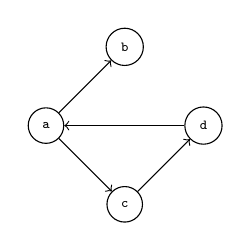
\begin{tikzpicture}
\node[draw, circle] (b) at (0, 0) {\tiny \texttt{b}};
\node[draw, circle] (a) at (-1, -1) {\tiny \texttt{a}};
\node[draw, circle] (d) at (1, -1) {\tiny \texttt{d}};
\node[draw, circle] (c) at (0, -2) {\tiny \texttt{c}};
\draw[->] (a) -- (b);
\draw[->] (a) -- (c);
\draw[->] (c) -- (d);
\draw[->] (d) -- (a);
\end{tikzpicture}
\end{center}
est repr\'{e}sent\'{e} par: \\

\noindent \texttt{link(a, b)}. \\
\texttt{link(a, c)}. \\
\texttt{link(c, d)}. \\
\texttt{link(d, a)}.

\begin{enumerate}
 \item \'{E}crivez un pr\'{e}dicat \texttt{path(X, Y)} qui est vrai s'il exsite un chemin de X \`{a} Y.
 \item Est-ce que l'ordre des pr\'{e}dicats dans votre programme a de l'importance?
 \item Comment calculer le chemin, et pas juste savoir s'il y en a un? Vous pouvez calculer le
 chemin dans l'ordre inverse si c'est plus simple.
 \item Comment on fait pour calculer tous les chemins entre X et Y?
\end{enumerate}

    \subsubsection*{Solution}
    \begin{enumerate}
    \item \textbf{TODO}
    \item \textbf{TODO}
    \item
    \begin{lstlisting}

    /* Partie 1 : Existence */

    link(a, b).
    link(a, c).
    link(c, d).
    link(d, a).

    path(X, Y) :- link(X, Y).
    path(X, Y) :- link(X, Z), path(Z, Y).

    /* Partie 2 : Ordre *

    path(X,Y) :- path(Z, Y), link(X, Z).
    %*\text{\% Fonctionne aussi, mais moins efficace.}*)
    %*\text{\% L’ordre des predicats n’a de l’importance que pour les performances.} *)

    /* Partie 3 : Chemin */

    link(a, b, [a, b]).
    link(a, c, [a, c]).
    link(c, d, [c, d]).

    path(X, Z, P) :- link(X, Z, P).
    path(X, Z, [X|P2]) :- link(X, Y, P1), path(Y, Z, P2).
    \end{lstlisting}

    \item Pour calculer tous les chemins, il suffit de lancer le programme de la partie 3, puis d'attendre une réponse.
    Lorsqu'on a une solution, on peut demander au programme de revenir en arrière et de modifier son dernier choix pour trouver une solution différente.
    En pratique, cela peut se faire en répondant à la réponse du programme par un ";" au lieu d'un ".".
    Il n'y a qu'à réitérer l'opération jusqu'à ce que le programme n'ait plus de choix disponible et qu'il se termine pour de bon.

   \end{enumerate}
\subsection*{Exercice 6}
Le programme suivant d\'{e}cide si un nombre est premier ou pas.

\begin{verbatim}
isPrime(2).
isPrime(3).
isPrime(P) :- P > 3, P mod 2 =\= 0, \+ hasFactor(P,3).
hasFactor(N,L) :- N mod L =:= 0.
hasFactor(N,L) :- L * L < N, L2 is L + 2, hasFactor(N,L2).
\end{verbatim}
Montrez les \'{e}tapes que prolog fait pour r\'{e}pondre aux requ\^{e}tes \texttt{isPrime(15)} et \texttt{isPrime(17)}.

    \subsubsection*{Solution}

    \begin{lstlisting}
    /* Requête initiale */
    r0 = < isPrime(15). >


    /* Résolution 1 */
    s1 = {(P, 15)}        % On sait que la variable P
                          % de la fonction isPrime vaut 15
    r1 = < 15>3, 15 mod 2 =\= 0, \+ hasFactor(15, 3). >
    % On developpe la fonction isPrime

    /* Résolution 2 */
    s2 = s1
    r2 = < 15 mod 2 =\= 0, \+ hasFactor(15, 3). >
    %15 est bien strictement superieur a 3

    /* Résolution 3 */
    s3 = s2
    r3 = < \+ hasFactor(15, 3). >
    %15 n'est pas divisible par 2

    /* Résolution 4 */
    s4 = s3 U {(L, 3)}     %On developpe hasFactor
    r4 = < \+ 3*3 < 15, L2 is 3+2, hasFactor(15, L2). >

    /* Résolution 5 */
    s5 = s4
    r5 = < \+ L2 is 3+2, hasFactor(15, L2). >

    /* Résolution 6 */
    s6 = s5 U {(L2, 5)}
    r6 = < \+ hasFactor(15, 5). >

    /* Résolution 7 */
    s7 = s6
    r7 = < \+ 15 mod 5 =:= 0. >
    %On passe dans le cas de base

    /* Résolution 8 */
    s8 = s7
    r8 = < \+ true >

    %La resolvante s'arrete car on a \+ true
    %(\+ implique que ce qui suit doit etre false)
    \end{lstlisting}

    \begin{lstlisting}
    /* Requête initiale */
    r0 = < isPrime(17). >


    /* Résolution 1 */
    s1 = {(P, 17)}        % Meme debut
    r1 = < 17>3, 17 mod 2 =\= 0, \+ hasFactor(17, 3). >

    /* Résolution 2 */
    s2 = s1
    r2 = < 17 mod 2 =\= 0, \+ hasFactor(17, 3). >

    /* Résolution 3 */
    s3 = s2
    r3 = < \+ hasFactor(17, 3). >

    /* Résolution 4 */
    s4 = s3 U {(L, 3)}     %On developpe hasFactor
    r4 = < \+ 3*3 < 17, L2 is 3+2, hasFactor(17, L2). >

    /* Résolution 5 */
    s5 = s4
    r5 = < \+ L2 is 3+2, hasFactor(17, L2). >

    /* Résolution 6 */
    s6 = s5 U {(L2, 5)}
    r6 = < \+ hasFactor(17, 5). >

    /* Résolution 7 */
    s7 = s6
    r7 = < \+ 5*5 < 17, L2' is 5+2, hasFactor(17, L2'). >
    %25 n'est pas inferieur a 17; false

    /* Résolution 8 */
    s8 = s7
    r8 = < \+ false >

    /* Résolution 9 */
    s9 = s8
    r9 = < >
    %La resolvante est vide
    %La requete renvoie true
    \end{lstlisting}

